\documentclass[a4paper, 12pt]{extarticle}
%------------------------------------------------------------------------------------
\usepackage[scaled]{helvet}
\renewcommand\familydefault{\sfdefault} 
\usepackage[T1]{fontenc}
\usepackage[english]{babel}
\usepackage{xargs}
\usepackage{graphicx}
\usepackage[pdftex,dvipsnames]{xcolor}
\usepackage{enumitem}
\usepackage{verbatim}
\usepackage{enumitem}
\usepackage{hyperref}
\usepackage[position=top]{subfig}
\usepackage{float}
\usepackage[none]{hyphenat}
\usepackage{longtable}
\usepackage[margin=1in]{geometry}
\usepackage{courier}
\usepackage{listings}
\lstset{basicstyle=\footnotesize\ttfamily,breaklines=true}
%------------------------------------------------------------------------------------

\begin{document}

\begin{titlepage}
	\centering
    
    {\normalsize 
        Professors Mottola Luca, Margara Alessandro\\
        \textbf{Middleware Technologies for Distributed Systems} \\ 
		Dipartimento di Elettronica, Informazione e Bioingegneria\\
		Politecnico di Milano \\\par
    }     
    \vspace{3cm}
    {\LARGE \textbf{Distributed Node-Red Flows} }
    \vspace{0.5cm}
    {\large \textbf{\\ Design document} \par}     
    \vspace{4cm}
	
\includegraphics[scale=0.4]{images/polimi.png}\\
	\vspace {3cm}
	
    {\normalsize 
	Luca Danelutti (10604455) \\ 
	Ian Di Dio Lavore (10580652)\\ 
	Gianmarco Tedeschi (10608433) \par
	}     
    
    \vspace{3cm}


	{\normalsize 29-09-2021 \par}
	
\end{titlepage}

\tableofcontents
\newpage

\section{Assignment}
\subsection{Scope}
You are to implement an architecture that allows Node-red flows to span multiple devices. Normally, a Node-red flow executes locally to the machine where it is installed.\\ Instead, consider multiple Node-red installations that:
\begin{itemize}
    \item register to a central repository that maintains information on all running installations
    \item can exchange messages among them by logically connecting the output of a node in one installation to the input of another node in a different installation 
\end{itemize}
Addressing of Node-red installations must be content-based, that is, the target Node-red installations that receive the messages cannot be determined based on their IP address or some other form of machine-level identifier. You need to demonstrate that a flow developed to be executed on a single Node-red installation may be split across two or multiple Node-red machines with a limited set of modifications to the flow itself.
\subsection{Assumptions and Guidelines}
\begin{enumerate}
    \item The project may be accomplished without creating custom nodes, that is, creating custom nodes is welcome but not mandatory.
\item The set of running Node-red installations is dynamic, that is, your implementation must be able to manage Node-red installations coming and going while the application executes.
\item Your solution must be agnostic to the content of messages, that is, it must be usable regardless of the format of messages or the nature of nodes that produce/consume them.
\end{enumerate}
\subsection{Technologies}
\begin{itemize}
    \item Node-red + one other technology of choice for the coordination among Node-red installations
\end{itemize}

\newpage

\section{Design choices}
\begin{figure*}[h]
    \centering
    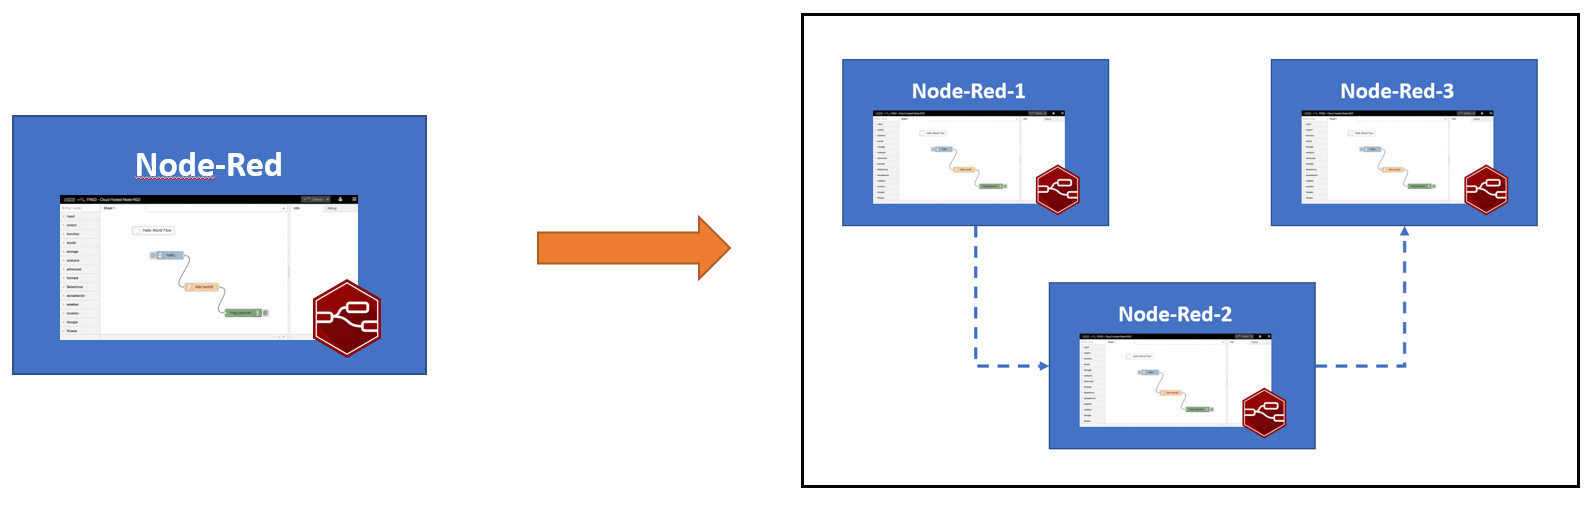
\includegraphics[width=\textwidth]{images/before_after.PNG}
    \captionof{figure}{Passing from a single flow to multiple connected flows}
    \label{fig:before-after}
\end{figure*}
We used KafkaJS inside of the custom nodes of Node-Red. Those nodes are able to communicate to a Kafka ecosystem. \\
The goal of the project was being able to divide an initial Node-Red flow into sub-elements that works independently on various machines. This is achieved by putting one of the custom nodes at the end of the first sub-flow and one at the beginning of the next sub-flow. 
The messages between flows are addressed by using topics that can be set by the user to the type of the message being produced (ex. "temp\_readings", "filtered\_output", etc. )


\subsection{Kafka}\label{kafka}
The text of the assignment clearly point us towards a technology that would have made possible to exchange messages without relying on the typical machine-level identifiers. The publish-subscribe pattern matched those indications and considering the technologies seen during the course (namely Contiki-NG, Node-red, Akka, Spark, Kafka, or MPI) our focus went into investigating the advantages of Akka over Kafka and vice-versa. 
We ended up using Kafka for the following reasons: 
\begin{itemize}
    \item Producers and consumers don't need to know each other and this allow us to comply to the requirement of no machine-level identifiers.
    \item Kafka handles the storing of unconsumed messages by itself, so consumers and producers don't need to be connected at all times. Kafka stores messages inside of topics that are stored on resilient memory (disk); Offsets are then used to replay messages if needed. 
    \item Kafka internally handle load-balancing by having partitions on the topics, those partitions can also be replicated to improve the fault-tolerance of the system.
    \item Kafka was chosen over Akka by the fact that we didn't need any computational power on the back-end system, we just needed a system that was designed to deliver messages. An Actor, the base unit of the Akka model, would have had its internal logic on how to respond to incoming messages.
    \item The requirement that the set of Node-Red installations is dynamic is also intrinsically addresses by the Kafka model, since producer and consumers are decoupled. 
\end{itemize}

\subsection{KafkaJS}\label{kafkajs}
This library is a connector between Kafka and Node.JS (the engine that runs Node-Red). It is rapidly growing traction among the community for its ease of use \href{https://github.com/tulios/kafkajs/issues/289}{[*]}.
\\
The library exposes three main components:
\begin{itemize}
    \item Client: it is the main connection point between Node.js and Kafka, handling the connection to the brokers and setting (almost) all the parameters exposed by Kafka. 
    \item Producer: this object is the element that will produce messages into Kafka topics
    \item Consumer: not surprisingly, this is the one that will consume messages
\end{itemize}
It is obviously mimicking the architecture of Kafka, to provide developers the same feeling as of Java/Scala.


\subsection{Node-Red}\label{node-red}
\begin{figure*}[h]
    \centering
    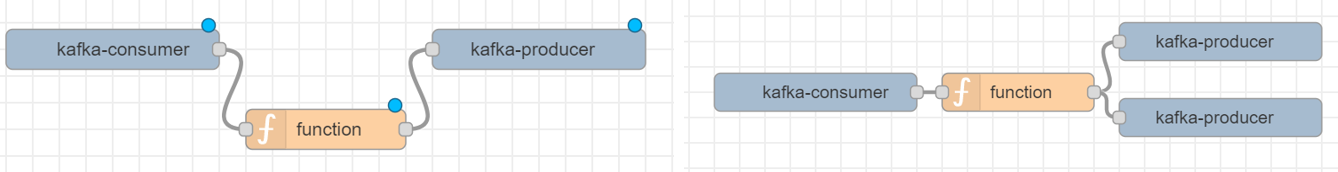
\includegraphics[width=\textwidth]{images/flows.PNG}
    \captionof{figure}{Custom nodes can be used in different configurations}
    \label{fig:flows}
\end{figure*}
We implemented a set of custom Node-Red nodes to provide the end-user an experience as smooth as possible. 
\begin{itemize}
    \item Kafka-producer
    \item Kafka-consumer 
\end{itemize}
The kafka-producer node has the option to set the topic where to send the messages.
On the other hand, kafka-consumer has also the setting for the groupID. The groupID is an option that will enable fault-tolerance of a single Node-Red by specifying the same groupID. A different groupID can be specified to split the flow into two branches.\\
An hidden configuration node was also built, to provide a unique connection to the Kafka brokers, this node was called Kafka-connection, but in KafkaJS terms it equals to the concept of Kafka client.
This node will provide the methods to create a new producer or consumer. It will take as input the clientID representing the current Node-Red flow and the initial broker list. 

\newpage
\section{Implementation}
In the figure below the setup used during the development is illustrated. 
We used Docker as our container engine and created a docker-compose.yml file to generate and run all the needed containers. A Dockerfile was also needed to create the image of Node-Red with the custom nodes pre-installed. 
\begin{figure*}[h]
    \centering
    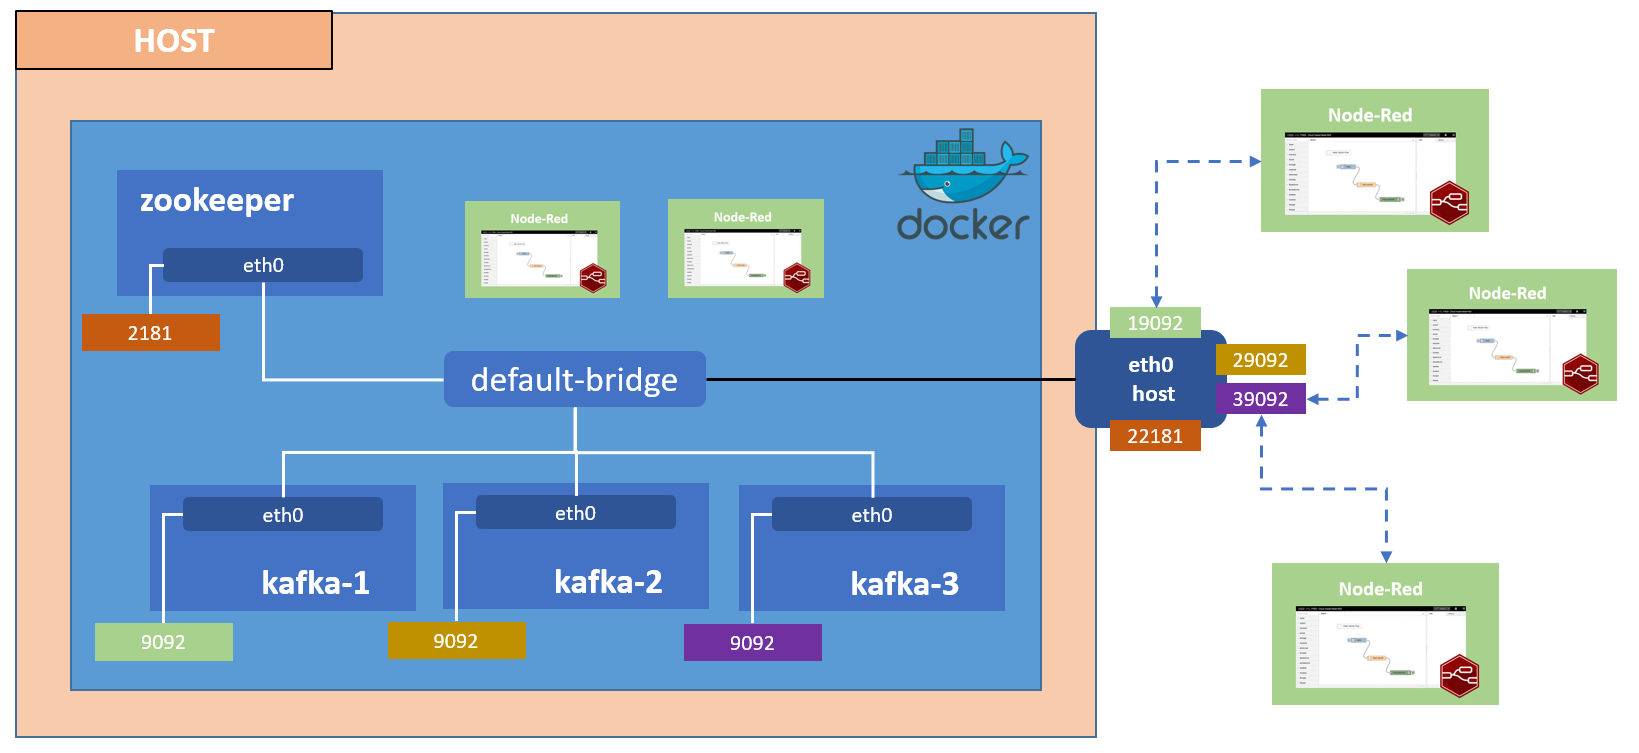
\includegraphics[width=\textwidth]{images/docker.PNG}
    \captionof{figure}{The setup used during the development and testing}
    \label{fig:docker}
\end{figure*}
\\
With proper modifications this setup can easily be extended on other scenarios.\\
By running the docker-compose.yml
\begin{lstlisting}[language=bash]
  $ docker-compose up -d
\end{lstlisting}
the following containers will start executing:
\begin{itemize}
    \item 3x Kafka (our Kafka cluster)
    \item 1x Zookeeper (the manager of the cluster)
    \item 3x Node-Red
\end{itemize}
The instances of Kafka and Zookeeper will also publish their port on the host interface to allow connection of external Node-Red servers and Kafka brokers.
The Node-Red containers are available at \lstinline{localhost:[1881,1882,1883]}.\\
To make the development and testing easier we used a web UI \href{https://github.com/provectus/kafka-ui}{[*]} (started together with the other containers) for monitoring and managing our Kafka cluster. This allowed us to both see messages generated/stored in topics and the consumers list with the topics assigned to them.

\newpage
\section{Notes and Improvements}
To successfully divide flows into sub-flows we must ensure that when a message exits one flow the receiving flow only receives exactly one message. Fortunately enough Kafka architecture with proper settings provides out of the box the exactly-once guarantees.\\
KafkaJS supports this feature only experimentally, we encountered some problems while testing the whole system and later discovered that it was due to this. 
An issue [\href{https://github.com/tulios/kafkajs/issues/598}{*}] on KafkaJS GitHub page is open to solve this problem and at the time of writing the developers seems to have fixed the cause but the new release is not available yet. \\
To temporarily solve this problem we implemented a HTTP POST request from within the failing node to restart the Node-Red flow. A more cleaner way would have been to disable the exactly-once semantic and check with an id inside of the message on the receiving side (the consumer) that the message wasn't already been serviced. \\
We used the default setting of KafkaJS to shard data over partitions which is in a round-robin fashion. We decided to go this way because in our mind the service that we offer to Node-Red should be as simple as possible to modify the flow into sub-flows. A small improvement on the system could be to enable the user to choose between the different settings exposed by KafkaJS.  

\section{References}
\begin{itemize}
\item \url{https://kafka.apache.org/}
\item \url{https://kafka.js.org/}
\item \url{https://nodered.org/}
\item \url{https://github.com/provectus/kafka-ui}
\item Lectures of Middleware Technologies of Distributed Systems - 052533 at PoliMi
\end{itemize}

\end{document}
    